% Created by tikzDevice version 0.12.6 on 2024-03-03 13:25:11
% !TEX encoding = UTF-8 Unicode
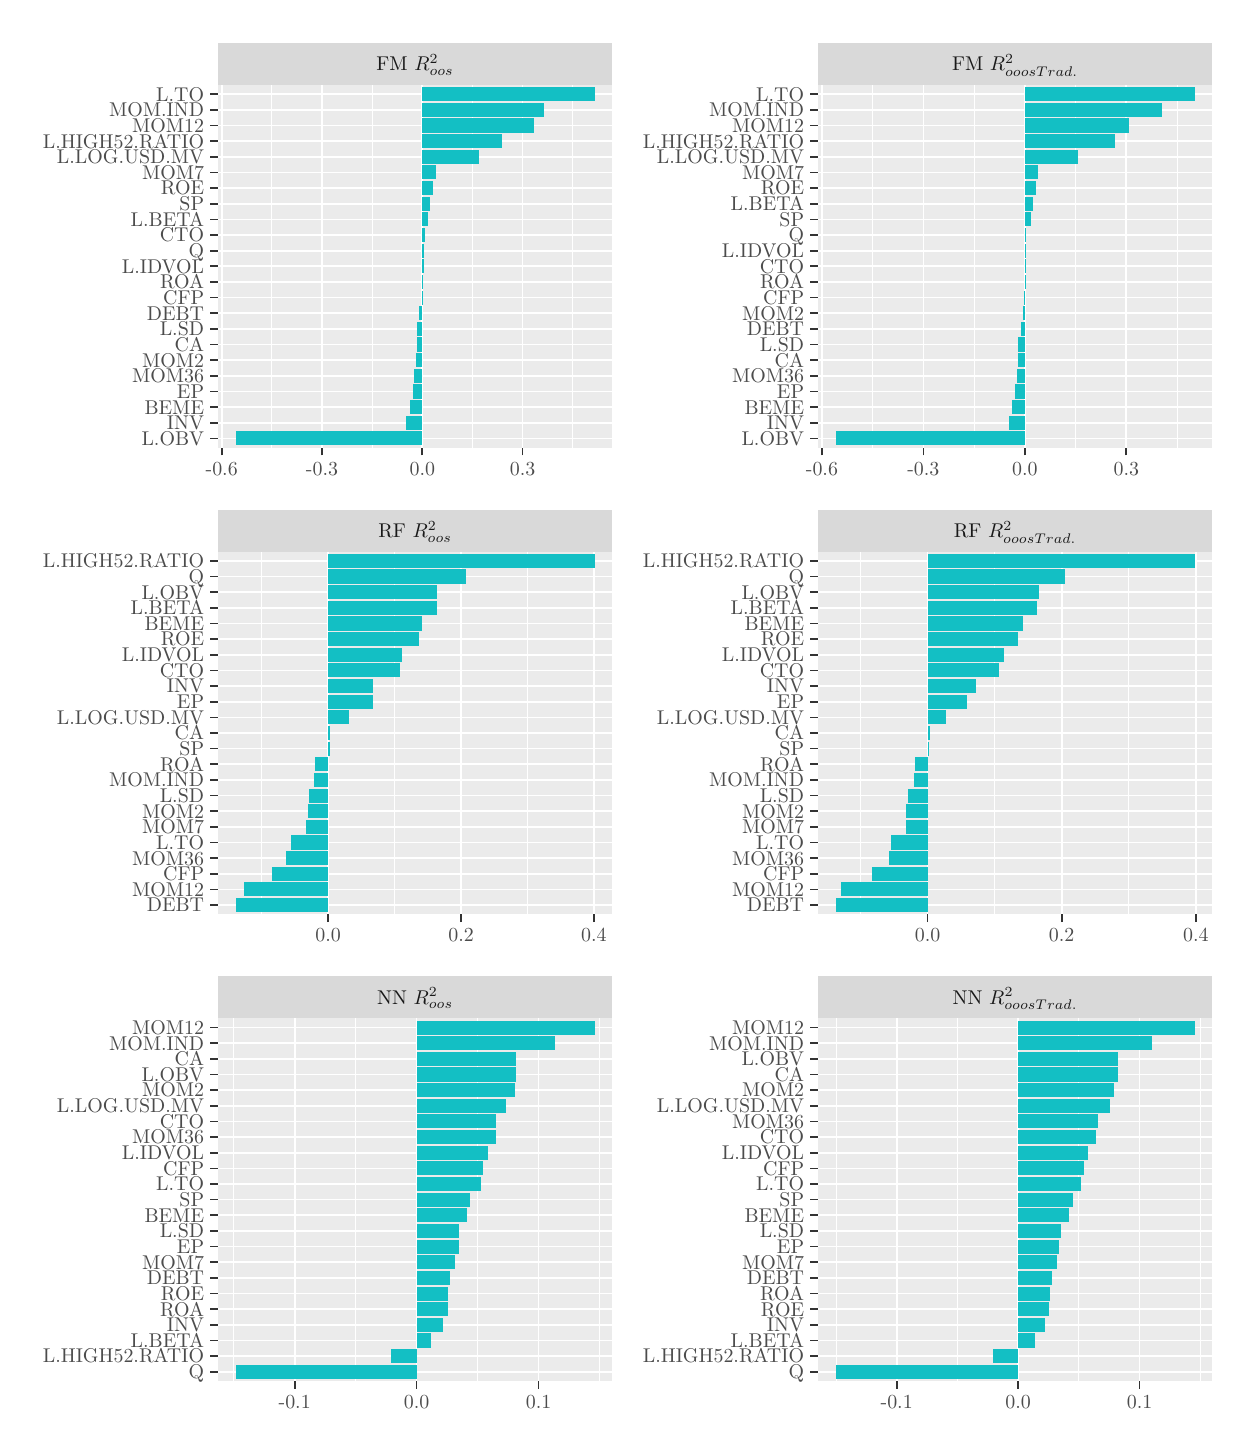
\begin{tikzpicture}[x=1pt,y=1pt]
\definecolor{fillColor}{RGB}{255,255,255}
\path[use as bounding box,fill=fillColor,fill opacity=0.00] (0,0) rectangle (433.62,505.89);
\begin{scope}
\path[clip] (  0.00,337.26) rectangle (216.81,505.89);
\definecolor{drawColor}{RGB}{255,255,255}
\definecolor{fillColor}{RGB}{255,255,255}

\path[draw=drawColor,line width= 0.6pt,line join=round,line cap=round,fill=fillColor] (  0.00,337.26) rectangle (216.81,505.89);
\end{scope}
\begin{scope}
\path[clip] ( 68.69,354.07) rectangle (211.31,485.23);
\definecolor{fillColor}{gray}{0.92}

\path[fill=fillColor] ( 68.69,354.07) rectangle (211.31,485.23);
\definecolor{drawColor}{RGB}{255,255,255}

\path[draw=drawColor,line width= 0.3pt,line join=round] ( 88.22,354.07) --
	( 88.22,485.23);

\path[draw=drawColor,line width= 0.3pt,line join=round] (124.47,354.07) --
	(124.47,485.23);

\path[draw=drawColor,line width= 0.3pt,line join=round] (160.71,354.07) --
	(160.71,485.23);

\path[draw=drawColor,line width= 0.3pt,line join=round] (196.95,354.07) --
	(196.95,485.23);

\path[draw=drawColor,line width= 0.6pt,line join=round] ( 68.69,357.46) --
	(211.31,357.46);

\path[draw=drawColor,line width= 0.6pt,line join=round] ( 68.69,363.11) --
	(211.31,363.11);

\path[draw=drawColor,line width= 0.6pt,line join=round] ( 68.69,368.77) --
	(211.31,368.77);

\path[draw=drawColor,line width= 0.6pt,line join=round] ( 68.69,374.42) --
	(211.31,374.42);

\path[draw=drawColor,line width= 0.6pt,line join=round] ( 68.69,380.07) --
	(211.31,380.07);

\path[draw=drawColor,line width= 0.6pt,line join=round] ( 68.69,385.73) --
	(211.31,385.73);

\path[draw=drawColor,line width= 0.6pt,line join=round] ( 68.69,391.38) --
	(211.31,391.38);

\path[draw=drawColor,line width= 0.6pt,line join=round] ( 68.69,397.04) --
	(211.31,397.04);

\path[draw=drawColor,line width= 0.6pt,line join=round] ( 68.69,402.69) --
	(211.31,402.69);

\path[draw=drawColor,line width= 0.6pt,line join=round] ( 68.69,408.34) --
	(211.31,408.34);

\path[draw=drawColor,line width= 0.6pt,line join=round] ( 68.69,414.00) --
	(211.31,414.00);

\path[draw=drawColor,line width= 0.6pt,line join=round] ( 68.69,419.65) --
	(211.31,419.65);

\path[draw=drawColor,line width= 0.6pt,line join=round] ( 68.69,425.30) --
	(211.31,425.30);

\path[draw=drawColor,line width= 0.6pt,line join=round] ( 68.69,430.96) --
	(211.31,430.96);

\path[draw=drawColor,line width= 0.6pt,line join=round] ( 68.69,436.61) --
	(211.31,436.61);

\path[draw=drawColor,line width= 0.6pt,line join=round] ( 68.69,442.26) --
	(211.31,442.26);

\path[draw=drawColor,line width= 0.6pt,line join=round] ( 68.69,447.92) --
	(211.31,447.92);

\path[draw=drawColor,line width= 0.6pt,line join=round] ( 68.69,453.57) --
	(211.31,453.57);

\path[draw=drawColor,line width= 0.6pt,line join=round] ( 68.69,459.23) --
	(211.31,459.23);

\path[draw=drawColor,line width= 0.6pt,line join=round] ( 68.69,464.88) --
	(211.31,464.88);

\path[draw=drawColor,line width= 0.6pt,line join=round] ( 68.69,470.53) --
	(211.31,470.53);

\path[draw=drawColor,line width= 0.6pt,line join=round] ( 68.69,476.19) --
	(211.31,476.19);

\path[draw=drawColor,line width= 0.6pt,line join=round] ( 68.69,481.84) --
	(211.31,481.84);

\path[draw=drawColor,line width= 0.6pt,line join=round] ( 70.10,354.07) --
	( 70.10,485.23);

\path[draw=drawColor,line width= 0.6pt,line join=round] (106.35,354.07) --
	(106.35,485.23);

\path[draw=drawColor,line width= 0.6pt,line join=round] (142.59,354.07) --
	(142.59,485.23);

\path[draw=drawColor,line width= 0.6pt,line join=round] (178.83,354.07) --
	(178.83,485.23);
\definecolor{fillColor}{RGB}{19,191,196}

\path[fill=fillColor] (140.72,388.84) rectangle (142.59,393.93);

\path[fill=fillColor] (142.59,428.41) rectangle (143.55,433.50);

\path[fill=fillColor] (138.11,366.22) rectangle (142.59,371.31);

\path[fill=fillColor] (142.59,405.80) rectangle (142.66,410.89);

\path[fill=fillColor] (136.82,360.57) rectangle (142.59,365.66);

\path[fill=fillColor] (141.57,400.15) rectangle (142.59,405.23);

\path[fill=fillColor] (142.59,439.72) rectangle (145.34,444.81);

\path[fill=fillColor] (139.18,371.88) rectangle (142.59,376.97);

\path[fill=fillColor] (142.59,411.45) rectangle (142.68,416.54);

\path[fill=fillColor] (142.59,445.37) rectangle (146.56,450.46);

\path[fill=fillColor] (142.59,422.76) rectangle (143.28,427.85);

\path[fill=fillColor] (142.59,451.03) rectangle (147.55,456.12);

\path[fill=fillColor] (142.59,467.99) rectangle (183.07,473.08);

\path[fill=fillColor] (139.54,377.53) rectangle (142.59,382.62);

\path[fill=fillColor] (140.17,383.18) rectangle (142.59,388.27);

\path[fill=fillColor] (142.59,473.64) rectangle (186.49,478.73);

\path[fill=fillColor] (140.85,394.49) rectangle (142.59,399.58);

\path[fill=fillColor] (142.59,462.33) rectangle (171.49,467.42);

\path[fill=fillColor] (142.59,434.07) rectangle (144.60,439.15);

\path[fill=fillColor] (142.59,417.11) rectangle (143.07,422.19);

\path[fill=fillColor] (142.59,456.68) rectangle (163.09,461.77);

\path[fill=fillColor] (142.59,479.30) rectangle (204.83,484.38);

\path[fill=fillColor] ( 75.17,354.92) rectangle (142.59,360.00);
\end{scope}
\begin{scope}
\path[clip] ( 68.69,485.23) rectangle (211.31,500.39);
\definecolor{fillColor}{gray}{0.85}

\path[fill=fillColor] ( 68.69,485.23) rectangle (211.31,500.39);
\definecolor{drawColor}{gray}{0.10}

\node[text=drawColor,anchor=base,inner sep=0pt, outer sep=0pt, scale=  0.72] at (140.00,490.33) {FM $R^2_{oos}$};
\end{scope}
\begin{scope}
\path[clip] (  0.00,  0.00) rectangle (433.62,505.89);
\definecolor{drawColor}{gray}{0.20}

\path[draw=drawColor,line width= 0.6pt,line join=round] ( 70.10,351.32) --
	( 70.10,354.07);

\path[draw=drawColor,line width= 0.6pt,line join=round] (106.35,351.32) --
	(106.35,354.07);

\path[draw=drawColor,line width= 0.6pt,line join=round] (142.59,351.32) --
	(142.59,354.07);

\path[draw=drawColor,line width= 0.6pt,line join=round] (178.83,351.32) --
	(178.83,354.07);
\end{scope}
\begin{scope}
\path[clip] (  0.00,  0.00) rectangle (433.62,505.89);
\definecolor{drawColor}{gray}{0.30}

\node[text=drawColor,anchor=base,inner sep=0pt, outer sep=0pt, scale=  0.72] at ( 70.10,344.16) {-0.6};

\node[text=drawColor,anchor=base,inner sep=0pt, outer sep=0pt, scale=  0.72] at (106.35,344.16) {-0.3};

\node[text=drawColor,anchor=base,inner sep=0pt, outer sep=0pt, scale=  0.72] at (142.59,344.16) {0.0};

\node[text=drawColor,anchor=base,inner sep=0pt, outer sep=0pt, scale=  0.72] at (178.83,344.16) {0.3};
\end{scope}
\begin{scope}
\path[clip] (  0.00,  0.00) rectangle (433.62,505.89);
\definecolor{drawColor}{gray}{0.30}

\node[text=drawColor,anchor=base east,inner sep=0pt, outer sep=0pt, scale=  0.72] at ( 63.74,354.98) {L.OBV};

\node[text=drawColor,anchor=base east,inner sep=0pt, outer sep=0pt, scale=  0.72] at ( 63.74,360.63) {INV};

\node[text=drawColor,anchor=base east,inner sep=0pt, outer sep=0pt, scale=  0.72] at ( 63.74,366.29) {BEME};

\node[text=drawColor,anchor=base east,inner sep=0pt, outer sep=0pt, scale=  0.72] at ( 63.74,371.94) {EP};

\node[text=drawColor,anchor=base east,inner sep=0pt, outer sep=0pt, scale=  0.72] at ( 63.74,377.60) {MOM36};

\node[text=drawColor,anchor=base east,inner sep=0pt, outer sep=0pt, scale=  0.72] at ( 63.74,383.25) {MOM2};

\node[text=drawColor,anchor=base east,inner sep=0pt, outer sep=0pt, scale=  0.72] at ( 63.74,388.90) {CA};

\node[text=drawColor,anchor=base east,inner sep=0pt, outer sep=0pt, scale=  0.72] at ( 63.74,394.56) {L.SD};

\node[text=drawColor,anchor=base east,inner sep=0pt, outer sep=0pt, scale=  0.72] at ( 63.74,400.21) {DEBT};

\node[text=drawColor,anchor=base east,inner sep=0pt, outer sep=0pt, scale=  0.72] at ( 63.74,405.86) {CFP};

\node[text=drawColor,anchor=base east,inner sep=0pt, outer sep=0pt, scale=  0.72] at ( 63.74,411.52) {ROA};

\node[text=drawColor,anchor=base east,inner sep=0pt, outer sep=0pt, scale=  0.72] at ( 63.74,417.17) {L.IDVOL};

\node[text=drawColor,anchor=base east,inner sep=0pt, outer sep=0pt, scale=  0.72] at ( 63.74,422.82) {Q};

\node[text=drawColor,anchor=base east,inner sep=0pt, outer sep=0pt, scale=  0.72] at ( 63.74,428.48) {CTO};

\node[text=drawColor,anchor=base east,inner sep=0pt, outer sep=0pt, scale=  0.72] at ( 63.74,434.13) {L.BETA};

\node[text=drawColor,anchor=base east,inner sep=0pt, outer sep=0pt, scale=  0.72] at ( 63.74,439.78) {SP};

\node[text=drawColor,anchor=base east,inner sep=0pt, outer sep=0pt, scale=  0.72] at ( 63.74,445.44) {ROE};

\node[text=drawColor,anchor=base east,inner sep=0pt, outer sep=0pt, scale=  0.72] at ( 63.74,451.09) {MOM7};

\node[text=drawColor,anchor=base east,inner sep=0pt, outer sep=0pt, scale=  0.72] at ( 63.74,456.75) {L.LOG.USD.MV};

\node[text=drawColor,anchor=base east,inner sep=0pt, outer sep=0pt, scale=  0.72] at ( 63.74,462.40) {L.HIGH52.RATIO};

\node[text=drawColor,anchor=base east,inner sep=0pt, outer sep=0pt, scale=  0.72] at ( 63.74,468.05) {MOM12};

\node[text=drawColor,anchor=base east,inner sep=0pt, outer sep=0pt, scale=  0.72] at ( 63.74,473.71) {MOM.IND};

\node[text=drawColor,anchor=base east,inner sep=0pt, outer sep=0pt, scale=  0.72] at ( 63.74,479.36) {L.TO};
\end{scope}
\begin{scope}
\path[clip] (  0.00,  0.00) rectangle (433.62,505.89);
\definecolor{drawColor}{gray}{0.20}

\path[draw=drawColor,line width= 0.6pt,line join=round] ( 65.94,357.46) --
	( 68.69,357.46);

\path[draw=drawColor,line width= 0.6pt,line join=round] ( 65.94,363.11) --
	( 68.69,363.11);

\path[draw=drawColor,line width= 0.6pt,line join=round] ( 65.94,368.77) --
	( 68.69,368.77);

\path[draw=drawColor,line width= 0.6pt,line join=round] ( 65.94,374.42) --
	( 68.69,374.42);

\path[draw=drawColor,line width= 0.6pt,line join=round] ( 65.94,380.07) --
	( 68.69,380.07);

\path[draw=drawColor,line width= 0.6pt,line join=round] ( 65.94,385.73) --
	( 68.69,385.73);

\path[draw=drawColor,line width= 0.6pt,line join=round] ( 65.94,391.38) --
	( 68.69,391.38);

\path[draw=drawColor,line width= 0.6pt,line join=round] ( 65.94,397.04) --
	( 68.69,397.04);

\path[draw=drawColor,line width= 0.6pt,line join=round] ( 65.94,402.69) --
	( 68.69,402.69);

\path[draw=drawColor,line width= 0.6pt,line join=round] ( 65.94,408.34) --
	( 68.69,408.34);

\path[draw=drawColor,line width= 0.6pt,line join=round] ( 65.94,414.00) --
	( 68.69,414.00);

\path[draw=drawColor,line width= 0.6pt,line join=round] ( 65.94,419.65) --
	( 68.69,419.65);

\path[draw=drawColor,line width= 0.6pt,line join=round] ( 65.94,425.30) --
	( 68.69,425.30);

\path[draw=drawColor,line width= 0.6pt,line join=round] ( 65.94,430.96) --
	( 68.69,430.96);

\path[draw=drawColor,line width= 0.6pt,line join=round] ( 65.94,436.61) --
	( 68.69,436.61);

\path[draw=drawColor,line width= 0.6pt,line join=round] ( 65.94,442.26) --
	( 68.69,442.26);

\path[draw=drawColor,line width= 0.6pt,line join=round] ( 65.94,447.92) --
	( 68.69,447.92);

\path[draw=drawColor,line width= 0.6pt,line join=round] ( 65.94,453.57) --
	( 68.69,453.57);

\path[draw=drawColor,line width= 0.6pt,line join=round] ( 65.94,459.23) --
	( 68.69,459.23);

\path[draw=drawColor,line width= 0.6pt,line join=round] ( 65.94,464.88) --
	( 68.69,464.88);

\path[draw=drawColor,line width= 0.6pt,line join=round] ( 65.94,470.53) --
	( 68.69,470.53);

\path[draw=drawColor,line width= 0.6pt,line join=round] ( 65.94,476.19) --
	( 68.69,476.19);

\path[draw=drawColor,line width= 0.6pt,line join=round] ( 65.94,481.84) --
	( 68.69,481.84);
\end{scope}
\begin{scope}
\path[clip] (216.81,337.26) rectangle (433.62,505.89);
\definecolor{drawColor}{RGB}{255,255,255}
\definecolor{fillColor}{RGB}{255,255,255}

\path[draw=drawColor,line width= 0.6pt,line join=round,line cap=round,fill=fillColor] (216.81,337.26) rectangle (433.62,505.89);
\end{scope}
\begin{scope}
\path[clip] (285.50,354.07) rectangle (428.12,485.23);
\definecolor{fillColor}{gray}{0.92}

\path[fill=fillColor] (285.50,354.07) rectangle (428.12,485.23);
\definecolor{drawColor}{RGB}{255,255,255}

\path[draw=drawColor,line width= 0.3pt,line join=round] (305.34,354.07) --
	(305.34,485.23);

\path[draw=drawColor,line width= 0.3pt,line join=round] (342.00,354.07) --
	(342.00,485.23);

\path[draw=drawColor,line width= 0.3pt,line join=round] (378.65,354.07) --
	(378.65,485.23);

\path[draw=drawColor,line width= 0.3pt,line join=round] (415.31,354.07) --
	(415.31,485.23);

\path[draw=drawColor,line width= 0.6pt,line join=round] (285.50,357.46) --
	(428.12,357.46);

\path[draw=drawColor,line width= 0.6pt,line join=round] (285.50,363.11) --
	(428.12,363.11);

\path[draw=drawColor,line width= 0.6pt,line join=round] (285.50,368.77) --
	(428.12,368.77);

\path[draw=drawColor,line width= 0.6pt,line join=round] (285.50,374.42) --
	(428.12,374.42);

\path[draw=drawColor,line width= 0.6pt,line join=round] (285.50,380.07) --
	(428.12,380.07);

\path[draw=drawColor,line width= 0.6pt,line join=round] (285.50,385.73) --
	(428.12,385.73);

\path[draw=drawColor,line width= 0.6pt,line join=round] (285.50,391.38) --
	(428.12,391.38);

\path[draw=drawColor,line width= 0.6pt,line join=round] (285.50,397.04) --
	(428.12,397.04);

\path[draw=drawColor,line width= 0.6pt,line join=round] (285.50,402.69) --
	(428.12,402.69);

\path[draw=drawColor,line width= 0.6pt,line join=round] (285.50,408.34) --
	(428.12,408.34);

\path[draw=drawColor,line width= 0.6pt,line join=round] (285.50,414.00) --
	(428.12,414.00);

\path[draw=drawColor,line width= 0.6pt,line join=round] (285.50,419.65) --
	(428.12,419.65);

\path[draw=drawColor,line width= 0.6pt,line join=round] (285.50,425.30) --
	(428.12,425.30);

\path[draw=drawColor,line width= 0.6pt,line join=round] (285.50,430.96) --
	(428.12,430.96);

\path[draw=drawColor,line width= 0.6pt,line join=round] (285.50,436.61) --
	(428.12,436.61);

\path[draw=drawColor,line width= 0.6pt,line join=round] (285.50,442.26) --
	(428.12,442.26);

\path[draw=drawColor,line width= 0.6pt,line join=round] (285.50,447.92) --
	(428.12,447.92);

\path[draw=drawColor,line width= 0.6pt,line join=round] (285.50,453.57) --
	(428.12,453.57);

\path[draw=drawColor,line width= 0.6pt,line join=round] (285.50,459.23) --
	(428.12,459.23);

\path[draw=drawColor,line width= 0.6pt,line join=round] (285.50,464.88) --
	(428.12,464.88);

\path[draw=drawColor,line width= 0.6pt,line join=round] (285.50,470.53) --
	(428.12,470.53);

\path[draw=drawColor,line width= 0.6pt,line join=round] (285.50,476.19) --
	(428.12,476.19);

\path[draw=drawColor,line width= 0.6pt,line join=round] (285.50,481.84) --
	(428.12,481.84);

\path[draw=drawColor,line width= 0.6pt,line join=round] (287.01,354.07) --
	(287.01,485.23);

\path[draw=drawColor,line width= 0.6pt,line join=round] (323.67,354.07) --
	(323.67,485.23);

\path[draw=drawColor,line width= 0.6pt,line join=round] (360.32,354.07) --
	(360.32,485.23);

\path[draw=drawColor,line width= 0.6pt,line join=round] (396.98,354.07) --
	(396.98,485.23);
\definecolor{fillColor}{RGB}{19,191,196}

\path[fill=fillColor] (357.75,383.18) rectangle (360.32,388.27);

\path[fill=fillColor] (360.32,417.11) rectangle (360.59,422.19);

\path[fill=fillColor] (355.56,366.22) rectangle (360.32,371.31);

\path[fill=fillColor] (360.05,405.80) rectangle (360.32,410.89);

\path[fill=fillColor] (354.46,360.57) rectangle (360.32,365.66);

\path[fill=fillColor] (358.80,394.49) rectangle (360.32,399.58);

\path[fill=fillColor] (360.32,434.07) rectangle (362.45,439.15);

\path[fill=fillColor] (356.74,371.88) rectangle (360.32,376.97);

\path[fill=fillColor] (360.32,411.45) rectangle (360.41,416.54);

\path[fill=fillColor] (360.32,445.37) rectangle (364.29,450.46);

\path[fill=fillColor] (360.32,428.41) rectangle (360.67,433.50);

\path[fill=fillColor] (360.32,451.03) rectangle (365.02,456.12);

\path[fill=fillColor] (360.32,467.99) rectangle (398.12,473.08);

\path[fill=fillColor] (357.59,377.53) rectangle (360.32,382.62);

\path[fill=fillColor] (359.59,400.15) rectangle (360.32,405.23);

\path[fill=fillColor] (360.32,473.64) rectangle (409.80,478.73);

\path[fill=fillColor] (357.82,388.84) rectangle (360.32,393.93);

\path[fill=fillColor] (360.32,462.33) rectangle (392.98,467.42);

\path[fill=fillColor] (360.32,439.72) rectangle (363.10,444.81);

\path[fill=fillColor] (360.32,422.76) rectangle (360.63,427.85);

\path[fill=fillColor] (360.32,456.68) rectangle (379.61,461.77);

\path[fill=fillColor] (360.32,479.30) rectangle (421.64,484.38);

\path[fill=fillColor] (291.98,354.92) rectangle (360.32,360.00);
\end{scope}
\begin{scope}
\path[clip] (285.50,485.23) rectangle (428.12,500.39);
\definecolor{fillColor}{gray}{0.85}

\path[fill=fillColor] (285.50,485.23) rectangle (428.12,500.39);
\definecolor{drawColor}{gray}{0.10}

\node[text=drawColor,anchor=base,inner sep=0pt, outer sep=0pt, scale=  0.72] at (356.81,490.33) {FM $R^2_{ooos  Trad.}$};
\end{scope}
\begin{scope}
\path[clip] (  0.00,  0.00) rectangle (433.62,505.89);
\definecolor{drawColor}{gray}{0.20}

\path[draw=drawColor,line width= 0.6pt,line join=round] (287.01,351.32) --
	(287.01,354.07);

\path[draw=drawColor,line width= 0.6pt,line join=round] (323.67,351.32) --
	(323.67,354.07);

\path[draw=drawColor,line width= 0.6pt,line join=round] (360.32,351.32) --
	(360.32,354.07);

\path[draw=drawColor,line width= 0.6pt,line join=round] (396.98,351.32) --
	(396.98,354.07);
\end{scope}
\begin{scope}
\path[clip] (  0.00,  0.00) rectangle (433.62,505.89);
\definecolor{drawColor}{gray}{0.30}

\node[text=drawColor,anchor=base,inner sep=0pt, outer sep=0pt, scale=  0.72] at (287.01,344.16) {-0.6};

\node[text=drawColor,anchor=base,inner sep=0pt, outer sep=0pt, scale=  0.72] at (323.67,344.16) {-0.3};

\node[text=drawColor,anchor=base,inner sep=0pt, outer sep=0pt, scale=  0.72] at (360.32,344.16) {0.0};

\node[text=drawColor,anchor=base,inner sep=0pt, outer sep=0pt, scale=  0.72] at (396.98,344.16) {0.3};
\end{scope}
\begin{scope}
\path[clip] (  0.00,  0.00) rectangle (433.62,505.89);
\definecolor{drawColor}{gray}{0.30}

\node[text=drawColor,anchor=base east,inner sep=0pt, outer sep=0pt, scale=  0.72] at (280.55,354.98) {L.OBV};

\node[text=drawColor,anchor=base east,inner sep=0pt, outer sep=0pt, scale=  0.72] at (280.55,360.63) {INV};

\node[text=drawColor,anchor=base east,inner sep=0pt, outer sep=0pt, scale=  0.72] at (280.55,366.29) {BEME};

\node[text=drawColor,anchor=base east,inner sep=0pt, outer sep=0pt, scale=  0.72] at (280.55,371.94) {EP};

\node[text=drawColor,anchor=base east,inner sep=0pt, outer sep=0pt, scale=  0.72] at (280.55,377.60) {MOM36};

\node[text=drawColor,anchor=base east,inner sep=0pt, outer sep=0pt, scale=  0.72] at (280.55,383.25) {CA};

\node[text=drawColor,anchor=base east,inner sep=0pt, outer sep=0pt, scale=  0.72] at (280.55,388.90) {L.SD};

\node[text=drawColor,anchor=base east,inner sep=0pt, outer sep=0pt, scale=  0.72] at (280.55,394.56) {DEBT};

\node[text=drawColor,anchor=base east,inner sep=0pt, outer sep=0pt, scale=  0.72] at (280.55,400.21) {MOM2};

\node[text=drawColor,anchor=base east,inner sep=0pt, outer sep=0pt, scale=  0.72] at (280.55,405.86) {CFP};

\node[text=drawColor,anchor=base east,inner sep=0pt, outer sep=0pt, scale=  0.72] at (280.55,411.52) {ROA};

\node[text=drawColor,anchor=base east,inner sep=0pt, outer sep=0pt, scale=  0.72] at (280.55,417.17) {CTO};

\node[text=drawColor,anchor=base east,inner sep=0pt, outer sep=0pt, scale=  0.72] at (280.55,422.82) {L.IDVOL};

\node[text=drawColor,anchor=base east,inner sep=0pt, outer sep=0pt, scale=  0.72] at (280.55,428.48) {Q};

\node[text=drawColor,anchor=base east,inner sep=0pt, outer sep=0pt, scale=  0.72] at (280.55,434.13) {SP};

\node[text=drawColor,anchor=base east,inner sep=0pt, outer sep=0pt, scale=  0.72] at (280.55,439.78) {L.BETA};

\node[text=drawColor,anchor=base east,inner sep=0pt, outer sep=0pt, scale=  0.72] at (280.55,445.44) {ROE};

\node[text=drawColor,anchor=base east,inner sep=0pt, outer sep=0pt, scale=  0.72] at (280.55,451.09) {MOM7};

\node[text=drawColor,anchor=base east,inner sep=0pt, outer sep=0pt, scale=  0.72] at (280.55,456.75) {L.LOG.USD.MV};

\node[text=drawColor,anchor=base east,inner sep=0pt, outer sep=0pt, scale=  0.72] at (280.55,462.40) {L.HIGH52.RATIO};

\node[text=drawColor,anchor=base east,inner sep=0pt, outer sep=0pt, scale=  0.72] at (280.55,468.05) {MOM12};

\node[text=drawColor,anchor=base east,inner sep=0pt, outer sep=0pt, scale=  0.72] at (280.55,473.71) {MOM.IND};

\node[text=drawColor,anchor=base east,inner sep=0pt, outer sep=0pt, scale=  0.72] at (280.55,479.36) {L.TO};
\end{scope}
\begin{scope}
\path[clip] (  0.00,  0.00) rectangle (433.62,505.89);
\definecolor{drawColor}{gray}{0.20}

\path[draw=drawColor,line width= 0.6pt,line join=round] (282.75,357.46) --
	(285.50,357.46);

\path[draw=drawColor,line width= 0.6pt,line join=round] (282.75,363.11) --
	(285.50,363.11);

\path[draw=drawColor,line width= 0.6pt,line join=round] (282.75,368.77) --
	(285.50,368.77);

\path[draw=drawColor,line width= 0.6pt,line join=round] (282.75,374.42) --
	(285.50,374.42);

\path[draw=drawColor,line width= 0.6pt,line join=round] (282.75,380.07) --
	(285.50,380.07);

\path[draw=drawColor,line width= 0.6pt,line join=round] (282.75,385.73) --
	(285.50,385.73);

\path[draw=drawColor,line width= 0.6pt,line join=round] (282.75,391.38) --
	(285.50,391.38);

\path[draw=drawColor,line width= 0.6pt,line join=round] (282.75,397.04) --
	(285.50,397.04);

\path[draw=drawColor,line width= 0.6pt,line join=round] (282.75,402.69) --
	(285.50,402.69);

\path[draw=drawColor,line width= 0.6pt,line join=round] (282.75,408.34) --
	(285.50,408.34);

\path[draw=drawColor,line width= 0.6pt,line join=round] (282.75,414.00) --
	(285.50,414.00);

\path[draw=drawColor,line width= 0.6pt,line join=round] (282.75,419.65) --
	(285.50,419.65);

\path[draw=drawColor,line width= 0.6pt,line join=round] (282.75,425.30) --
	(285.50,425.30);

\path[draw=drawColor,line width= 0.6pt,line join=round] (282.75,430.96) --
	(285.50,430.96);

\path[draw=drawColor,line width= 0.6pt,line join=round] (282.75,436.61) --
	(285.50,436.61);

\path[draw=drawColor,line width= 0.6pt,line join=round] (282.75,442.26) --
	(285.50,442.26);

\path[draw=drawColor,line width= 0.6pt,line join=round] (282.75,447.92) --
	(285.50,447.92);

\path[draw=drawColor,line width= 0.6pt,line join=round] (282.75,453.57) --
	(285.50,453.57);

\path[draw=drawColor,line width= 0.6pt,line join=round] (282.75,459.23) --
	(285.50,459.23);

\path[draw=drawColor,line width= 0.6pt,line join=round] (282.75,464.88) --
	(285.50,464.88);

\path[draw=drawColor,line width= 0.6pt,line join=round] (282.75,470.53) --
	(285.50,470.53);

\path[draw=drawColor,line width= 0.6pt,line join=round] (282.75,476.19) --
	(285.50,476.19);

\path[draw=drawColor,line width= 0.6pt,line join=round] (282.75,481.84) --
	(285.50,481.84);
\end{scope}
\begin{scope}
\path[clip] (  0.00,168.63) rectangle (216.81,337.26);
\definecolor{drawColor}{RGB}{255,255,255}
\definecolor{fillColor}{RGB}{255,255,255}

\path[draw=drawColor,line width= 0.6pt,line join=round,line cap=round,fill=fillColor] (  0.00,168.63) rectangle (216.81,337.26);
\end{scope}
\begin{scope}
\path[clip] ( 68.69,185.44) rectangle (211.31,316.60);
\definecolor{fillColor}{gray}{0.92}

\path[fill=fillColor] ( 68.69,185.44) rectangle (211.31,316.60);
\definecolor{drawColor}{RGB}{255,255,255}

\path[draw=drawColor,line width= 0.3pt,line join=round] ( 84.61,185.44) --
	( 84.61,316.60);

\path[draw=drawColor,line width= 0.3pt,line join=round] (132.60,185.44) --
	(132.60,316.60);

\path[draw=drawColor,line width= 0.3pt,line join=round] (180.60,185.44) --
	(180.60,316.60);

\path[draw=drawColor,line width= 0.6pt,line join=round] ( 68.69,188.83) --
	(211.31,188.83);

\path[draw=drawColor,line width= 0.6pt,line join=round] ( 68.69,194.48) --
	(211.31,194.48);

\path[draw=drawColor,line width= 0.6pt,line join=round] ( 68.69,200.14) --
	(211.31,200.14);

\path[draw=drawColor,line width= 0.6pt,line join=round] ( 68.69,205.79) --
	(211.31,205.79);

\path[draw=drawColor,line width= 0.6pt,line join=round] ( 68.69,211.44) --
	(211.31,211.44);

\path[draw=drawColor,line width= 0.6pt,line join=round] ( 68.69,217.10) --
	(211.31,217.10);

\path[draw=drawColor,line width= 0.6pt,line join=round] ( 68.69,222.75) --
	(211.31,222.75);

\path[draw=drawColor,line width= 0.6pt,line join=round] ( 68.69,228.41) --
	(211.31,228.41);

\path[draw=drawColor,line width= 0.6pt,line join=round] ( 68.69,234.06) --
	(211.31,234.06);

\path[draw=drawColor,line width= 0.6pt,line join=round] ( 68.69,239.71) --
	(211.31,239.71);

\path[draw=drawColor,line width= 0.6pt,line join=round] ( 68.69,245.37) --
	(211.31,245.37);

\path[draw=drawColor,line width= 0.6pt,line join=round] ( 68.69,251.02) --
	(211.31,251.02);

\path[draw=drawColor,line width= 0.6pt,line join=round] ( 68.69,256.67) --
	(211.31,256.67);

\path[draw=drawColor,line width= 0.6pt,line join=round] ( 68.69,262.33) --
	(211.31,262.33);

\path[draw=drawColor,line width= 0.6pt,line join=round] ( 68.69,267.98) --
	(211.31,267.98);

\path[draw=drawColor,line width= 0.6pt,line join=round] ( 68.69,273.63) --
	(211.31,273.63);

\path[draw=drawColor,line width= 0.6pt,line join=round] ( 68.69,279.29) --
	(211.31,279.29);

\path[draw=drawColor,line width= 0.6pt,line join=round] ( 68.69,284.94) --
	(211.31,284.94);

\path[draw=drawColor,line width= 0.6pt,line join=round] ( 68.69,290.60) --
	(211.31,290.60);

\path[draw=drawColor,line width= 0.6pt,line join=round] ( 68.69,296.25) --
	(211.31,296.25);

\path[draw=drawColor,line width= 0.6pt,line join=round] ( 68.69,301.90) --
	(211.31,301.90);

\path[draw=drawColor,line width= 0.6pt,line join=round] ( 68.69,307.56) --
	(211.31,307.56);

\path[draw=drawColor,line width= 0.6pt,line join=round] ( 68.69,313.21) --
	(211.31,313.21);

\path[draw=drawColor,line width= 0.6pt,line join=round] (108.60,185.44) --
	(108.60,316.60);

\path[draw=drawColor,line width= 0.6pt,line join=round] (156.60,185.44) --
	(156.60,316.60);

\path[draw=drawColor,line width= 0.6pt,line join=round] (204.59,185.44) --
	(204.59,316.60);
\definecolor{fillColor}{RGB}{19,191,196}

\path[fill=fillColor] (108.60,248.48) rectangle (109.41,253.56);

\path[fill=fillColor] (108.60,271.09) rectangle (134.41,276.18);

\path[fill=fillColor] (108.60,288.05) rectangle (142.44,293.14);

\path[fill=fillColor] ( 88.33,197.59) rectangle (108.60,202.68);

\path[fill=fillColor] (108.60,265.44) rectangle (124.87,270.52);

\path[fill=fillColor] ( 75.17,186.29) rectangle (108.60,191.37);

\path[fill=fillColor] (108.60,242.82) rectangle (109.33,247.91);

\path[fill=fillColor] (108.60,259.78) rectangle (124.63,264.87);

\path[fill=fillColor] (103.79,237.17) rectangle (108.60,242.26);

\path[fill=fillColor] (108.60,282.40) rectangle (141.58,287.49);

\path[fill=fillColor] (108.60,305.01) rectangle (158.41,310.10);

\path[fill=fillColor] (100.44,214.55) rectangle (108.60,219.64);

\path[fill=fillColor] ( 78.00,191.94) rectangle (108.60,197.03);

\path[fill=fillColor] ( 93.41,203.25) rectangle (108.60,208.34);

\path[fill=fillColor] (101.20,220.21) rectangle (108.60,225.30);

\path[fill=fillColor] (103.51,231.52) rectangle (108.60,236.60);

\path[fill=fillColor] (101.58,225.86) rectangle (108.60,230.95);

\path[fill=fillColor] (108.60,310.67) rectangle (204.83,315.75);

\path[fill=fillColor] (108.60,293.70) rectangle (147.95,298.79);

\path[fill=fillColor] (108.60,276.74) rectangle (135.33,281.83);

\path[fill=fillColor] (108.60,254.13) rectangle (116.15,259.22);

\path[fill=fillColor] ( 95.12,208.90) rectangle (108.60,213.99);

\path[fill=fillColor] (108.60,299.36) rectangle (147.97,304.45);
\end{scope}
\begin{scope}
\path[clip] ( 68.69,316.60) rectangle (211.31,331.76);
\definecolor{fillColor}{gray}{0.85}

\path[fill=fillColor] ( 68.69,316.60) rectangle (211.31,331.76);
\definecolor{drawColor}{gray}{0.10}

\node[text=drawColor,anchor=base,inner sep=0pt, outer sep=0pt, scale=  0.72] at (140.00,321.70) {RF $R^2_{oos}$};
\end{scope}
\begin{scope}
\path[clip] (  0.00,  0.00) rectangle (433.62,505.89);
\definecolor{drawColor}{gray}{0.20}

\path[draw=drawColor,line width= 0.6pt,line join=round] (108.60,182.69) --
	(108.60,185.44);

\path[draw=drawColor,line width= 0.6pt,line join=round] (156.60,182.69) --
	(156.60,185.44);

\path[draw=drawColor,line width= 0.6pt,line join=round] (204.59,182.69) --
	(204.59,185.44);
\end{scope}
\begin{scope}
\path[clip] (  0.00,  0.00) rectangle (433.62,505.89);
\definecolor{drawColor}{gray}{0.30}

\node[text=drawColor,anchor=base,inner sep=0pt, outer sep=0pt, scale=  0.72] at (108.60,175.53) {0.0};

\node[text=drawColor,anchor=base,inner sep=0pt, outer sep=0pt, scale=  0.72] at (156.60,175.53) {0.2};

\node[text=drawColor,anchor=base,inner sep=0pt, outer sep=0pt, scale=  0.72] at (204.59,175.53) {0.4};
\end{scope}
\begin{scope}
\path[clip] (  0.00,  0.00) rectangle (433.62,505.89);
\definecolor{drawColor}{gray}{0.30}

\node[text=drawColor,anchor=base east,inner sep=0pt, outer sep=0pt, scale=  0.72] at ( 63.74,186.35) {DEBT};

\node[text=drawColor,anchor=base east,inner sep=0pt, outer sep=0pt, scale=  0.72] at ( 63.74,192.00) {MOM12};

\node[text=drawColor,anchor=base east,inner sep=0pt, outer sep=0pt, scale=  0.72] at ( 63.74,197.66) {CFP};

\node[text=drawColor,anchor=base east,inner sep=0pt, outer sep=0pt, scale=  0.72] at ( 63.74,203.31) {MOM36};

\node[text=drawColor,anchor=base east,inner sep=0pt, outer sep=0pt, scale=  0.72] at ( 63.74,208.97) {L.TO};

\node[text=drawColor,anchor=base east,inner sep=0pt, outer sep=0pt, scale=  0.72] at ( 63.74,214.62) {MOM7};

\node[text=drawColor,anchor=base east,inner sep=0pt, outer sep=0pt, scale=  0.72] at ( 63.74,220.27) {MOM2};

\node[text=drawColor,anchor=base east,inner sep=0pt, outer sep=0pt, scale=  0.72] at ( 63.74,225.93) {L.SD};

\node[text=drawColor,anchor=base east,inner sep=0pt, outer sep=0pt, scale=  0.72] at ( 63.74,231.58) {MOM.IND};

\node[text=drawColor,anchor=base east,inner sep=0pt, outer sep=0pt, scale=  0.72] at ( 63.74,237.23) {ROA};

\node[text=drawColor,anchor=base east,inner sep=0pt, outer sep=0pt, scale=  0.72] at ( 63.74,242.89) {SP};

\node[text=drawColor,anchor=base east,inner sep=0pt, outer sep=0pt, scale=  0.72] at ( 63.74,248.54) {CA};

\node[text=drawColor,anchor=base east,inner sep=0pt, outer sep=0pt, scale=  0.72] at ( 63.74,254.19) {L.LOG.USD.MV};

\node[text=drawColor,anchor=base east,inner sep=0pt, outer sep=0pt, scale=  0.72] at ( 63.74,259.85) {EP};

\node[text=drawColor,anchor=base east,inner sep=0pt, outer sep=0pt, scale=  0.72] at ( 63.74,265.50) {INV};

\node[text=drawColor,anchor=base east,inner sep=0pt, outer sep=0pt, scale=  0.72] at ( 63.74,271.15) {CTO};

\node[text=drawColor,anchor=base east,inner sep=0pt, outer sep=0pt, scale=  0.72] at ( 63.74,276.81) {L.IDVOL};

\node[text=drawColor,anchor=base east,inner sep=0pt, outer sep=0pt, scale=  0.72] at ( 63.74,282.46) {ROE};

\node[text=drawColor,anchor=base east,inner sep=0pt, outer sep=0pt, scale=  0.72] at ( 63.74,288.12) {BEME};

\node[text=drawColor,anchor=base east,inner sep=0pt, outer sep=0pt, scale=  0.72] at ( 63.74,293.77) {L.BETA};

\node[text=drawColor,anchor=base east,inner sep=0pt, outer sep=0pt, scale=  0.72] at ( 63.74,299.42) {L.OBV};

\node[text=drawColor,anchor=base east,inner sep=0pt, outer sep=0pt, scale=  0.72] at ( 63.74,305.08) {Q};

\node[text=drawColor,anchor=base east,inner sep=0pt, outer sep=0pt, scale=  0.72] at ( 63.74,310.73) {L.HIGH52.RATIO};
\end{scope}
\begin{scope}
\path[clip] (  0.00,  0.00) rectangle (433.62,505.89);
\definecolor{drawColor}{gray}{0.20}

\path[draw=drawColor,line width= 0.6pt,line join=round] ( 65.94,188.83) --
	( 68.69,188.83);

\path[draw=drawColor,line width= 0.6pt,line join=round] ( 65.94,194.48) --
	( 68.69,194.48);

\path[draw=drawColor,line width= 0.6pt,line join=round] ( 65.94,200.14) --
	( 68.69,200.14);

\path[draw=drawColor,line width= 0.6pt,line join=round] ( 65.94,205.79) --
	( 68.69,205.79);

\path[draw=drawColor,line width= 0.6pt,line join=round] ( 65.94,211.44) --
	( 68.69,211.44);

\path[draw=drawColor,line width= 0.6pt,line join=round] ( 65.94,217.10) --
	( 68.69,217.10);

\path[draw=drawColor,line width= 0.6pt,line join=round] ( 65.94,222.75) --
	( 68.69,222.75);

\path[draw=drawColor,line width= 0.6pt,line join=round] ( 65.94,228.41) --
	( 68.69,228.41);

\path[draw=drawColor,line width= 0.6pt,line join=round] ( 65.94,234.06) --
	( 68.69,234.06);

\path[draw=drawColor,line width= 0.6pt,line join=round] ( 65.94,239.71) --
	( 68.69,239.71);

\path[draw=drawColor,line width= 0.6pt,line join=round] ( 65.94,245.37) --
	( 68.69,245.37);

\path[draw=drawColor,line width= 0.6pt,line join=round] ( 65.94,251.02) --
	( 68.69,251.02);

\path[draw=drawColor,line width= 0.6pt,line join=round] ( 65.94,256.67) --
	( 68.69,256.67);

\path[draw=drawColor,line width= 0.6pt,line join=round] ( 65.94,262.33) --
	( 68.69,262.33);

\path[draw=drawColor,line width= 0.6pt,line join=round] ( 65.94,267.98) --
	( 68.69,267.98);

\path[draw=drawColor,line width= 0.6pt,line join=round] ( 65.94,273.63) --
	( 68.69,273.63);

\path[draw=drawColor,line width= 0.6pt,line join=round] ( 65.94,279.29) --
	( 68.69,279.29);

\path[draw=drawColor,line width= 0.6pt,line join=round] ( 65.94,284.94) --
	( 68.69,284.94);

\path[draw=drawColor,line width= 0.6pt,line join=round] ( 65.94,290.60) --
	( 68.69,290.60);

\path[draw=drawColor,line width= 0.6pt,line join=round] ( 65.94,296.25) --
	( 68.69,296.25);

\path[draw=drawColor,line width= 0.6pt,line join=round] ( 65.94,301.90) --
	( 68.69,301.90);

\path[draw=drawColor,line width= 0.6pt,line join=round] ( 65.94,307.56) --
	( 68.69,307.56);

\path[draw=drawColor,line width= 0.6pt,line join=round] ( 65.94,313.21) --
	( 68.69,313.21);
\end{scope}
\begin{scope}
\path[clip] (216.81,168.63) rectangle (433.62,337.26);
\definecolor{drawColor}{RGB}{255,255,255}
\definecolor{fillColor}{RGB}{255,255,255}

\path[draw=drawColor,line width= 0.6pt,line join=round,line cap=round,fill=fillColor] (216.81,168.63) rectangle (433.62,337.26);
\end{scope}
\begin{scope}
\path[clip] (285.50,185.44) rectangle (428.12,316.60);
\definecolor{fillColor}{gray}{0.92}

\path[fill=fillColor] (285.50,185.44) rectangle (428.12,316.60);
\definecolor{drawColor}{RGB}{255,255,255}

\path[draw=drawColor,line width= 0.3pt,line join=round] (300.94,185.44) --
	(300.94,316.60);

\path[draw=drawColor,line width= 0.3pt,line join=round] (349.40,185.44) --
	(349.40,316.60);

\path[draw=drawColor,line width= 0.3pt,line join=round] (397.87,185.44) --
	(397.87,316.60);

\path[draw=drawColor,line width= 0.6pt,line join=round] (285.50,188.83) --
	(428.12,188.83);

\path[draw=drawColor,line width= 0.6pt,line join=round] (285.50,194.48) --
	(428.12,194.48);

\path[draw=drawColor,line width= 0.6pt,line join=round] (285.50,200.14) --
	(428.12,200.14);

\path[draw=drawColor,line width= 0.6pt,line join=round] (285.50,205.79) --
	(428.12,205.79);

\path[draw=drawColor,line width= 0.6pt,line join=round] (285.50,211.44) --
	(428.12,211.44);

\path[draw=drawColor,line width= 0.6pt,line join=round] (285.50,217.10) --
	(428.12,217.10);

\path[draw=drawColor,line width= 0.6pt,line join=round] (285.50,222.75) --
	(428.12,222.75);

\path[draw=drawColor,line width= 0.6pt,line join=round] (285.50,228.41) --
	(428.12,228.41);

\path[draw=drawColor,line width= 0.6pt,line join=round] (285.50,234.06) --
	(428.12,234.06);

\path[draw=drawColor,line width= 0.6pt,line join=round] (285.50,239.71) --
	(428.12,239.71);

\path[draw=drawColor,line width= 0.6pt,line join=round] (285.50,245.37) --
	(428.12,245.37);

\path[draw=drawColor,line width= 0.6pt,line join=round] (285.50,251.02) --
	(428.12,251.02);

\path[draw=drawColor,line width= 0.6pt,line join=round] (285.50,256.67) --
	(428.12,256.67);

\path[draw=drawColor,line width= 0.6pt,line join=round] (285.50,262.33) --
	(428.12,262.33);

\path[draw=drawColor,line width= 0.6pt,line join=round] (285.50,267.98) --
	(428.12,267.98);

\path[draw=drawColor,line width= 0.6pt,line join=round] (285.50,273.63) --
	(428.12,273.63);

\path[draw=drawColor,line width= 0.6pt,line join=round] (285.50,279.29) --
	(428.12,279.29);

\path[draw=drawColor,line width= 0.6pt,line join=round] (285.50,284.94) --
	(428.12,284.94);

\path[draw=drawColor,line width= 0.6pt,line join=round] (285.50,290.60) --
	(428.12,290.60);

\path[draw=drawColor,line width= 0.6pt,line join=round] (285.50,296.25) --
	(428.12,296.25);

\path[draw=drawColor,line width= 0.6pt,line join=round] (285.50,301.90) --
	(428.12,301.90);

\path[draw=drawColor,line width= 0.6pt,line join=round] (285.50,307.56) --
	(428.12,307.56);

\path[draw=drawColor,line width= 0.6pt,line join=round] (285.50,313.21) --
	(428.12,313.21);

\path[draw=drawColor,line width= 0.6pt,line join=round] (325.17,185.44) --
	(325.17,316.60);

\path[draw=drawColor,line width= 0.6pt,line join=round] (373.64,185.44) --
	(373.64,316.60);

\path[draw=drawColor,line width= 0.6pt,line join=round] (422.10,185.44) --
	(422.10,316.60);
\definecolor{fillColor}{RGB}{19,191,196}

\path[fill=fillColor] (325.17,248.48) rectangle (326.20,253.56);

\path[fill=fillColor] (325.17,271.09) rectangle (351.15,276.18);

\path[fill=fillColor] (325.17,288.05) rectangle (359.70,293.14);

\path[fill=fillColor] (304.92,197.59) rectangle (325.17,202.68);

\path[fill=fillColor] (325.17,265.44) rectangle (342.66,270.52);

\path[fill=fillColor] (291.98,186.29) rectangle (325.17,191.37);

\path[fill=fillColor] (325.17,242.82) rectangle (325.62,247.91);

\path[fill=fillColor] (325.17,259.78) rectangle (339.35,264.87);

\path[fill=fillColor] (320.65,237.17) rectangle (325.17,242.26);

\path[fill=fillColor] (325.17,282.40) rectangle (357.71,287.49);

\path[fill=fillColor] (325.17,305.01) rectangle (374.77,310.10);

\path[fill=fillColor] (317.41,214.55) rectangle (325.17,219.64);

\path[fill=fillColor] (293.75,191.94) rectangle (325.17,197.03);

\path[fill=fillColor] (311.28,203.25) rectangle (325.17,208.34);

\path[fill=fillColor] (317.44,220.21) rectangle (325.17,225.30);

\path[fill=fillColor] (320.22,231.52) rectangle (325.17,236.60);

\path[fill=fillColor] (317.96,225.86) rectangle (325.17,230.95);

\path[fill=fillColor] (325.17,310.67) rectangle (421.64,315.75);

\path[fill=fillColor] (325.17,293.70) rectangle (364.83,298.79);

\path[fill=fillColor] (325.17,276.74) rectangle (352.72,281.83);

\path[fill=fillColor] (325.17,254.13) rectangle (331.93,259.22);

\path[fill=fillColor] (312.09,208.90) rectangle (325.17,213.99);

\path[fill=fillColor] (325.17,299.36) rectangle (365.32,304.45);
\end{scope}
\begin{scope}
\path[clip] (285.50,316.60) rectangle (428.12,331.76);
\definecolor{fillColor}{gray}{0.85}

\path[fill=fillColor] (285.50,316.60) rectangle (428.12,331.76);
\definecolor{drawColor}{gray}{0.10}

\node[text=drawColor,anchor=base,inner sep=0pt, outer sep=0pt, scale=  0.72] at (356.81,321.70) {RF $R^2_{ooos  Trad.}$};
\end{scope}
\begin{scope}
\path[clip] (  0.00,  0.00) rectangle (433.62,505.89);
\definecolor{drawColor}{gray}{0.20}

\path[draw=drawColor,line width= 0.6pt,line join=round] (325.17,182.69) --
	(325.17,185.44);

\path[draw=drawColor,line width= 0.6pt,line join=round] (373.64,182.69) --
	(373.64,185.44);

\path[draw=drawColor,line width= 0.6pt,line join=round] (422.10,182.69) --
	(422.10,185.44);
\end{scope}
\begin{scope}
\path[clip] (  0.00,  0.00) rectangle (433.62,505.89);
\definecolor{drawColor}{gray}{0.30}

\node[text=drawColor,anchor=base,inner sep=0pt, outer sep=0pt, scale=  0.72] at (325.17,175.53) {0.0};

\node[text=drawColor,anchor=base,inner sep=0pt, outer sep=0pt, scale=  0.72] at (373.64,175.53) {0.2};

\node[text=drawColor,anchor=base,inner sep=0pt, outer sep=0pt, scale=  0.72] at (422.10,175.53) {0.4};
\end{scope}
\begin{scope}
\path[clip] (  0.00,  0.00) rectangle (433.62,505.89);
\definecolor{drawColor}{gray}{0.30}

\node[text=drawColor,anchor=base east,inner sep=0pt, outer sep=0pt, scale=  0.72] at (280.55,186.35) {DEBT};

\node[text=drawColor,anchor=base east,inner sep=0pt, outer sep=0pt, scale=  0.72] at (280.55,192.00) {MOM12};

\node[text=drawColor,anchor=base east,inner sep=0pt, outer sep=0pt, scale=  0.72] at (280.55,197.66) {CFP};

\node[text=drawColor,anchor=base east,inner sep=0pt, outer sep=0pt, scale=  0.72] at (280.55,203.31) {MOM36};

\node[text=drawColor,anchor=base east,inner sep=0pt, outer sep=0pt, scale=  0.72] at (280.55,208.97) {L.TO};

\node[text=drawColor,anchor=base east,inner sep=0pt, outer sep=0pt, scale=  0.72] at (280.55,214.62) {MOM7};

\node[text=drawColor,anchor=base east,inner sep=0pt, outer sep=0pt, scale=  0.72] at (280.55,220.27) {MOM2};

\node[text=drawColor,anchor=base east,inner sep=0pt, outer sep=0pt, scale=  0.72] at (280.55,225.93) {L.SD};

\node[text=drawColor,anchor=base east,inner sep=0pt, outer sep=0pt, scale=  0.72] at (280.55,231.58) {MOM.IND};

\node[text=drawColor,anchor=base east,inner sep=0pt, outer sep=0pt, scale=  0.72] at (280.55,237.23) {ROA};

\node[text=drawColor,anchor=base east,inner sep=0pt, outer sep=0pt, scale=  0.72] at (280.55,242.89) {SP};

\node[text=drawColor,anchor=base east,inner sep=0pt, outer sep=0pt, scale=  0.72] at (280.55,248.54) {CA};

\node[text=drawColor,anchor=base east,inner sep=0pt, outer sep=0pt, scale=  0.72] at (280.55,254.19) {L.LOG.USD.MV};

\node[text=drawColor,anchor=base east,inner sep=0pt, outer sep=0pt, scale=  0.72] at (280.55,259.85) {EP};

\node[text=drawColor,anchor=base east,inner sep=0pt, outer sep=0pt, scale=  0.72] at (280.55,265.50) {INV};

\node[text=drawColor,anchor=base east,inner sep=0pt, outer sep=0pt, scale=  0.72] at (280.55,271.15) {CTO};

\node[text=drawColor,anchor=base east,inner sep=0pt, outer sep=0pt, scale=  0.72] at (280.55,276.81) {L.IDVOL};

\node[text=drawColor,anchor=base east,inner sep=0pt, outer sep=0pt, scale=  0.72] at (280.55,282.46) {ROE};

\node[text=drawColor,anchor=base east,inner sep=0pt, outer sep=0pt, scale=  0.72] at (280.55,288.12) {BEME};

\node[text=drawColor,anchor=base east,inner sep=0pt, outer sep=0pt, scale=  0.72] at (280.55,293.77) {L.BETA};

\node[text=drawColor,anchor=base east,inner sep=0pt, outer sep=0pt, scale=  0.72] at (280.55,299.42) {L.OBV};

\node[text=drawColor,anchor=base east,inner sep=0pt, outer sep=0pt, scale=  0.72] at (280.55,305.08) {Q};

\node[text=drawColor,anchor=base east,inner sep=0pt, outer sep=0pt, scale=  0.72] at (280.55,310.73) {L.HIGH52.RATIO};
\end{scope}
\begin{scope}
\path[clip] (  0.00,  0.00) rectangle (433.62,505.89);
\definecolor{drawColor}{gray}{0.20}

\path[draw=drawColor,line width= 0.6pt,line join=round] (282.75,188.83) --
	(285.50,188.83);

\path[draw=drawColor,line width= 0.6pt,line join=round] (282.75,194.48) --
	(285.50,194.48);

\path[draw=drawColor,line width= 0.6pt,line join=round] (282.75,200.14) --
	(285.50,200.14);

\path[draw=drawColor,line width= 0.6pt,line join=round] (282.75,205.79) --
	(285.50,205.79);

\path[draw=drawColor,line width= 0.6pt,line join=round] (282.75,211.44) --
	(285.50,211.44);

\path[draw=drawColor,line width= 0.6pt,line join=round] (282.75,217.10) --
	(285.50,217.10);

\path[draw=drawColor,line width= 0.6pt,line join=round] (282.75,222.75) --
	(285.50,222.75);

\path[draw=drawColor,line width= 0.6pt,line join=round] (282.75,228.41) --
	(285.50,228.41);

\path[draw=drawColor,line width= 0.6pt,line join=round] (282.75,234.06) --
	(285.50,234.06);

\path[draw=drawColor,line width= 0.6pt,line join=round] (282.75,239.71) --
	(285.50,239.71);

\path[draw=drawColor,line width= 0.6pt,line join=round] (282.75,245.37) --
	(285.50,245.37);

\path[draw=drawColor,line width= 0.6pt,line join=round] (282.75,251.02) --
	(285.50,251.02);

\path[draw=drawColor,line width= 0.6pt,line join=round] (282.75,256.67) --
	(285.50,256.67);

\path[draw=drawColor,line width= 0.6pt,line join=round] (282.75,262.33) --
	(285.50,262.33);

\path[draw=drawColor,line width= 0.6pt,line join=round] (282.75,267.98) --
	(285.50,267.98);

\path[draw=drawColor,line width= 0.6pt,line join=round] (282.75,273.63) --
	(285.50,273.63);

\path[draw=drawColor,line width= 0.6pt,line join=round] (282.75,279.29) --
	(285.50,279.29);

\path[draw=drawColor,line width= 0.6pt,line join=round] (282.75,284.94) --
	(285.50,284.94);

\path[draw=drawColor,line width= 0.6pt,line join=round] (282.75,290.60) --
	(285.50,290.60);

\path[draw=drawColor,line width= 0.6pt,line join=round] (282.75,296.25) --
	(285.50,296.25);

\path[draw=drawColor,line width= 0.6pt,line join=round] (282.75,301.90) --
	(285.50,301.90);

\path[draw=drawColor,line width= 0.6pt,line join=round] (282.75,307.56) --
	(285.50,307.56);

\path[draw=drawColor,line width= 0.6pt,line join=round] (282.75,313.21) --
	(285.50,313.21);
\end{scope}
\begin{scope}
\path[clip] (  0.00,  0.00) rectangle (216.81,168.63);
\definecolor{drawColor}{RGB}{255,255,255}
\definecolor{fillColor}{RGB}{255,255,255}

\path[draw=drawColor,line width= 0.6pt,line join=round,line cap=round,fill=fillColor] (  0.00,  0.00) rectangle (216.81,168.63);
\end{scope}
\begin{scope}
\path[clip] ( 68.69, 16.81) rectangle (211.31,147.97);
\definecolor{fillColor}{gray}{0.92}

\path[fill=fillColor] ( 68.69, 16.81) rectangle (211.31,147.97);
\definecolor{drawColor}{RGB}{255,255,255}

\path[draw=drawColor,line width= 0.3pt,line join=round] ( 74.45, 16.81) --
	( 74.45,147.97);

\path[draw=drawColor,line width= 0.3pt,line join=round] (118.52, 16.81) --
	(118.52,147.97);

\path[draw=drawColor,line width= 0.3pt,line join=round] (162.60, 16.81) --
	(162.60,147.97);

\path[draw=drawColor,line width= 0.3pt,line join=round] (206.67, 16.81) --
	(206.67,147.97);

\path[draw=drawColor,line width= 0.6pt,line join=round] ( 68.69, 20.20) --
	(211.31, 20.20);

\path[draw=drawColor,line width= 0.6pt,line join=round] ( 68.69, 25.85) --
	(211.31, 25.85);

\path[draw=drawColor,line width= 0.6pt,line join=round] ( 68.69, 31.51) --
	(211.31, 31.51);

\path[draw=drawColor,line width= 0.6pt,line join=round] ( 68.69, 37.16) --
	(211.31, 37.16);

\path[draw=drawColor,line width= 0.6pt,line join=round] ( 68.69, 42.81) --
	(211.31, 42.81);

\path[draw=drawColor,line width= 0.6pt,line join=round] ( 68.69, 48.47) --
	(211.31, 48.47);

\path[draw=drawColor,line width= 0.6pt,line join=round] ( 68.69, 54.12) --
	(211.31, 54.12);

\path[draw=drawColor,line width= 0.6pt,line join=round] ( 68.69, 59.78) --
	(211.31, 59.78);

\path[draw=drawColor,line width= 0.6pt,line join=round] ( 68.69, 65.43) --
	(211.31, 65.43);

\path[draw=drawColor,line width= 0.6pt,line join=round] ( 68.69, 71.08) --
	(211.31, 71.08);

\path[draw=drawColor,line width= 0.6pt,line join=round] ( 68.69, 76.74) --
	(211.31, 76.74);

\path[draw=drawColor,line width= 0.6pt,line join=round] ( 68.69, 82.39) --
	(211.31, 82.39);

\path[draw=drawColor,line width= 0.6pt,line join=round] ( 68.69, 88.04) --
	(211.31, 88.04);

\path[draw=drawColor,line width= 0.6pt,line join=round] ( 68.69, 93.70) --
	(211.31, 93.70);

\path[draw=drawColor,line width= 0.6pt,line join=round] ( 68.69, 99.35) --
	(211.31, 99.35);

\path[draw=drawColor,line width= 0.6pt,line join=round] ( 68.69,105.00) --
	(211.31,105.00);

\path[draw=drawColor,line width= 0.6pt,line join=round] ( 68.69,110.66) --
	(211.31,110.66);

\path[draw=drawColor,line width= 0.6pt,line join=round] ( 68.69,116.31) --
	(211.31,116.31);

\path[draw=drawColor,line width= 0.6pt,line join=round] ( 68.69,121.97) --
	(211.31,121.97);

\path[draw=drawColor,line width= 0.6pt,line join=round] ( 68.69,127.62) --
	(211.31,127.62);

\path[draw=drawColor,line width= 0.6pt,line join=round] ( 68.69,133.27) --
	(211.31,133.27);

\path[draw=drawColor,line width= 0.6pt,line join=round] ( 68.69,138.93) --
	(211.31,138.93);

\path[draw=drawColor,line width= 0.6pt,line join=round] ( 68.69,144.58) --
	(211.31,144.58);

\path[draw=drawColor,line width= 0.6pt,line join=round] ( 96.48, 16.81) --
	( 96.48,147.97);

\path[draw=drawColor,line width= 0.6pt,line join=round] (140.56, 16.81) --
	(140.56,147.97);

\path[draw=drawColor,line width= 0.6pt,line join=round] (184.63, 16.81) --
	(184.63,147.97);
\definecolor{fillColor}{RGB}{19,191,196}

\path[fill=fillColor] (140.56,130.73) rectangle (176.56,135.82);

\path[fill=fillColor] (140.56,108.11) rectangle (169.31,113.20);

\path[fill=fillColor] (140.56, 74.19) rectangle (158.61, 79.28);

\path[fill=fillColor] (140.56, 91.15) rectangle (164.69, 96.24);

\path[fill=fillColor] (140.56, 34.62) rectangle (150.14, 39.71);

\path[fill=fillColor] (140.56, 51.58) rectangle (152.51, 56.67);

\path[fill=fillColor] (140.56, 79.85) rectangle (160.01, 84.93);

\path[fill=fillColor] (140.56, 62.89) rectangle (155.73, 67.97);

\path[fill=fillColor] (140.56, 40.27) rectangle (151.99, 45.36);

\path[fill=fillColor] (140.56, 45.92) rectangle (152.00, 51.01);

\path[fill=fillColor] ( 75.17, 17.66) rectangle (140.56, 22.74);

\path[fill=fillColor] (140.56, 57.23) rectangle (154.46, 62.32);

\path[fill=fillColor] (140.56,142.04) rectangle (204.83,147.12);

\path[fill=fillColor] (140.56,102.46) rectangle (169.11,107.55);

\path[fill=fillColor] (140.56,119.42) rectangle (176.03,124.51);

\path[fill=fillColor] (140.56,136.38) rectangle (190.60,141.47);

\path[fill=fillColor] (140.56, 68.54) rectangle (155.86, 73.63);

\path[fill=fillColor] (131.18, 23.31) rectangle (140.56, 28.40);

\path[fill=fillColor] (140.56, 28.96) rectangle (145.72, 34.05);

\path[fill=fillColor] (140.56, 96.81) rectangle (166.21,101.89);

\path[fill=fillColor] (140.56,113.77) rectangle (172.85,118.86);

\path[fill=fillColor] (140.56, 85.50) rectangle (163.63, 90.59);

\path[fill=fillColor] (140.56,125.07) rectangle (176.38,130.16);
\end{scope}
\begin{scope}
\path[clip] ( 68.69,147.97) rectangle (211.31,163.13);
\definecolor{fillColor}{gray}{0.85}

\path[fill=fillColor] ( 68.69,147.97) rectangle (211.31,163.13);
\definecolor{drawColor}{gray}{0.10}

\node[text=drawColor,anchor=base,inner sep=0pt, outer sep=0pt, scale=  0.72] at (140.00,153.07) {NN $R^2_{oos}$};
\end{scope}
\begin{scope}
\path[clip] (  0.00,  0.00) rectangle (433.62,505.89);
\definecolor{drawColor}{gray}{0.20}

\path[draw=drawColor,line width= 0.6pt,line join=round] ( 96.48, 14.06) --
	( 96.48, 16.81);

\path[draw=drawColor,line width= 0.6pt,line join=round] (140.56, 14.06) --
	(140.56, 16.81);

\path[draw=drawColor,line width= 0.6pt,line join=round] (184.63, 14.06) --
	(184.63, 16.81);
\end{scope}
\begin{scope}
\path[clip] (  0.00,  0.00) rectangle (433.62,505.89);
\definecolor{drawColor}{gray}{0.30}

\node[text=drawColor,anchor=base,inner sep=0pt, outer sep=0pt, scale=  0.72] at ( 96.48,  6.90) {-0.1};

\node[text=drawColor,anchor=base,inner sep=0pt, outer sep=0pt, scale=  0.72] at (140.56,  6.90) {0.0};

\node[text=drawColor,anchor=base,inner sep=0pt, outer sep=0pt, scale=  0.72] at (184.63,  6.90) {0.1};
\end{scope}
\begin{scope}
\path[clip] (  0.00,  0.00) rectangle (433.62,505.89);
\definecolor{drawColor}{gray}{0.30}

\node[text=drawColor,anchor=base east,inner sep=0pt, outer sep=0pt, scale=  0.72] at ( 63.74, 17.72) {Q};

\node[text=drawColor,anchor=base east,inner sep=0pt, outer sep=0pt, scale=  0.72] at ( 63.74, 23.37) {L.HIGH52.RATIO};

\node[text=drawColor,anchor=base east,inner sep=0pt, outer sep=0pt, scale=  0.72] at ( 63.74, 29.03) {L.BETA};

\node[text=drawColor,anchor=base east,inner sep=0pt, outer sep=0pt, scale=  0.72] at ( 63.74, 34.68) {INV};

\node[text=drawColor,anchor=base east,inner sep=0pt, outer sep=0pt, scale=  0.72] at ( 63.74, 40.34) {ROA};

\node[text=drawColor,anchor=base east,inner sep=0pt, outer sep=0pt, scale=  0.72] at ( 63.74, 45.99) {ROE};

\node[text=drawColor,anchor=base east,inner sep=0pt, outer sep=0pt, scale=  0.72] at ( 63.74, 51.64) {DEBT};

\node[text=drawColor,anchor=base east,inner sep=0pt, outer sep=0pt, scale=  0.72] at ( 63.74, 57.30) {MOM7};

\node[text=drawColor,anchor=base east,inner sep=0pt, outer sep=0pt, scale=  0.72] at ( 63.74, 62.95) {EP};

\node[text=drawColor,anchor=base east,inner sep=0pt, outer sep=0pt, scale=  0.72] at ( 63.74, 68.60) {L.SD};

\node[text=drawColor,anchor=base east,inner sep=0pt, outer sep=0pt, scale=  0.72] at ( 63.74, 74.26) {BEME};

\node[text=drawColor,anchor=base east,inner sep=0pt, outer sep=0pt, scale=  0.72] at ( 63.74, 79.91) {SP};

\node[text=drawColor,anchor=base east,inner sep=0pt, outer sep=0pt, scale=  0.72] at ( 63.74, 85.56) {L.TO};

\node[text=drawColor,anchor=base east,inner sep=0pt, outer sep=0pt, scale=  0.72] at ( 63.74, 91.22) {CFP};

\node[text=drawColor,anchor=base east,inner sep=0pt, outer sep=0pt, scale=  0.72] at ( 63.74, 96.87) {L.IDVOL};

\node[text=drawColor,anchor=base east,inner sep=0pt, outer sep=0pt, scale=  0.72] at ( 63.74,102.52) {MOM36};

\node[text=drawColor,anchor=base east,inner sep=0pt, outer sep=0pt, scale=  0.72] at ( 63.74,108.18) {CTO};

\node[text=drawColor,anchor=base east,inner sep=0pt, outer sep=0pt, scale=  0.72] at ( 63.74,113.83) {L.LOG.USD.MV};

\node[text=drawColor,anchor=base east,inner sep=0pt, outer sep=0pt, scale=  0.72] at ( 63.74,119.49) {MOM2};

\node[text=drawColor,anchor=base east,inner sep=0pt, outer sep=0pt, scale=  0.72] at ( 63.74,125.14) {L.OBV};

\node[text=drawColor,anchor=base east,inner sep=0pt, outer sep=0pt, scale=  0.72] at ( 63.74,130.79) {CA};

\node[text=drawColor,anchor=base east,inner sep=0pt, outer sep=0pt, scale=  0.72] at ( 63.74,136.45) {MOM.IND};

\node[text=drawColor,anchor=base east,inner sep=0pt, outer sep=0pt, scale=  0.72] at ( 63.74,142.10) {MOM12};
\end{scope}
\begin{scope}
\path[clip] (  0.00,  0.00) rectangle (433.62,505.89);
\definecolor{drawColor}{gray}{0.20}

\path[draw=drawColor,line width= 0.6pt,line join=round] ( 65.94, 20.20) --
	( 68.69, 20.20);

\path[draw=drawColor,line width= 0.6pt,line join=round] ( 65.94, 25.85) --
	( 68.69, 25.85);

\path[draw=drawColor,line width= 0.6pt,line join=round] ( 65.94, 31.51) --
	( 68.69, 31.51);

\path[draw=drawColor,line width= 0.6pt,line join=round] ( 65.94, 37.16) --
	( 68.69, 37.16);

\path[draw=drawColor,line width= 0.6pt,line join=round] ( 65.94, 42.81) --
	( 68.69, 42.81);

\path[draw=drawColor,line width= 0.6pt,line join=round] ( 65.94, 48.47) --
	( 68.69, 48.47);

\path[draw=drawColor,line width= 0.6pt,line join=round] ( 65.94, 54.12) --
	( 68.69, 54.12);

\path[draw=drawColor,line width= 0.6pt,line join=round] ( 65.94, 59.78) --
	( 68.69, 59.78);

\path[draw=drawColor,line width= 0.6pt,line join=round] ( 65.94, 65.43) --
	( 68.69, 65.43);

\path[draw=drawColor,line width= 0.6pt,line join=round] ( 65.94, 71.08) --
	( 68.69, 71.08);

\path[draw=drawColor,line width= 0.6pt,line join=round] ( 65.94, 76.74) --
	( 68.69, 76.74);

\path[draw=drawColor,line width= 0.6pt,line join=round] ( 65.94, 82.39) --
	( 68.69, 82.39);

\path[draw=drawColor,line width= 0.6pt,line join=round] ( 65.94, 88.04) --
	( 68.69, 88.04);

\path[draw=drawColor,line width= 0.6pt,line join=round] ( 65.94, 93.70) --
	( 68.69, 93.70);

\path[draw=drawColor,line width= 0.6pt,line join=round] ( 65.94, 99.35) --
	( 68.69, 99.35);

\path[draw=drawColor,line width= 0.6pt,line join=round] ( 65.94,105.00) --
	( 68.69,105.00);

\path[draw=drawColor,line width= 0.6pt,line join=round] ( 65.94,110.66) --
	( 68.69,110.66);

\path[draw=drawColor,line width= 0.6pt,line join=round] ( 65.94,116.31) --
	( 68.69,116.31);

\path[draw=drawColor,line width= 0.6pt,line join=round] ( 65.94,121.97) --
	( 68.69,121.97);

\path[draw=drawColor,line width= 0.6pt,line join=round] ( 65.94,127.62) --
	( 68.69,127.62);

\path[draw=drawColor,line width= 0.6pt,line join=round] ( 65.94,133.27) --
	( 68.69,133.27);

\path[draw=drawColor,line width= 0.6pt,line join=round] ( 65.94,138.93) --
	( 68.69,138.93);

\path[draw=drawColor,line width= 0.6pt,line join=round] ( 65.94,144.58) --
	( 68.69,144.58);
\end{scope}
\begin{scope}
\path[clip] (216.81,  0.00) rectangle (433.62,168.63);
\definecolor{drawColor}{RGB}{255,255,255}
\definecolor{fillColor}{RGB}{255,255,255}

\path[draw=drawColor,line width= 0.6pt,line join=round,line cap=round,fill=fillColor] (216.81,  0.00) rectangle (433.62,168.63);
\end{scope}
\begin{scope}
\path[clip] (285.50, 16.81) rectangle (428.12,147.97);
\definecolor{fillColor}{gray}{0.92}

\path[fill=fillColor] (285.50, 16.81) rectangle (428.12,147.97);
\definecolor{drawColor}{RGB}{255,255,255}

\path[draw=drawColor,line width= 0.3pt,line join=round] (292.06, 16.81) --
	(292.06,147.97);

\path[draw=drawColor,line width= 0.3pt,line join=round] (335.96, 16.81) --
	(335.96,147.97);

\path[draw=drawColor,line width= 0.3pt,line join=round] (379.85, 16.81) --
	(379.85,147.97);

\path[draw=drawColor,line width= 0.3pt,line join=round] (423.74, 16.81) --
	(423.74,147.97);

\path[draw=drawColor,line width= 0.6pt,line join=round] (285.50, 20.20) --
	(428.12, 20.20);

\path[draw=drawColor,line width= 0.6pt,line join=round] (285.50, 25.85) --
	(428.12, 25.85);

\path[draw=drawColor,line width= 0.6pt,line join=round] (285.50, 31.51) --
	(428.12, 31.51);

\path[draw=drawColor,line width= 0.6pt,line join=round] (285.50, 37.16) --
	(428.12, 37.16);

\path[draw=drawColor,line width= 0.6pt,line join=round] (285.50, 42.81) --
	(428.12, 42.81);

\path[draw=drawColor,line width= 0.6pt,line join=round] (285.50, 48.47) --
	(428.12, 48.47);

\path[draw=drawColor,line width= 0.6pt,line join=round] (285.50, 54.12) --
	(428.12, 54.12);

\path[draw=drawColor,line width= 0.6pt,line join=round] (285.50, 59.78) --
	(428.12, 59.78);

\path[draw=drawColor,line width= 0.6pt,line join=round] (285.50, 65.43) --
	(428.12, 65.43);

\path[draw=drawColor,line width= 0.6pt,line join=round] (285.50, 71.08) --
	(428.12, 71.08);

\path[draw=drawColor,line width= 0.6pt,line join=round] (285.50, 76.74) --
	(428.12, 76.74);

\path[draw=drawColor,line width= 0.6pt,line join=round] (285.50, 82.39) --
	(428.12, 82.39);

\path[draw=drawColor,line width= 0.6pt,line join=round] (285.50, 88.04) --
	(428.12, 88.04);

\path[draw=drawColor,line width= 0.6pt,line join=round] (285.50, 93.70) --
	(428.12, 93.70);

\path[draw=drawColor,line width= 0.6pt,line join=round] (285.50, 99.35) --
	(428.12, 99.35);

\path[draw=drawColor,line width= 0.6pt,line join=round] (285.50,105.00) --
	(428.12,105.00);

\path[draw=drawColor,line width= 0.6pt,line join=round] (285.50,110.66) --
	(428.12,110.66);

\path[draw=drawColor,line width= 0.6pt,line join=round] (285.50,116.31) --
	(428.12,116.31);

\path[draw=drawColor,line width= 0.6pt,line join=round] (285.50,121.97) --
	(428.12,121.97);

\path[draw=drawColor,line width= 0.6pt,line join=round] (285.50,127.62) --
	(428.12,127.62);

\path[draw=drawColor,line width= 0.6pt,line join=round] (285.50,133.27) --
	(428.12,133.27);

\path[draw=drawColor,line width= 0.6pt,line join=round] (285.50,138.93) --
	(428.12,138.93);

\path[draw=drawColor,line width= 0.6pt,line join=round] (285.50,144.58) --
	(428.12,144.58);

\path[draw=drawColor,line width= 0.6pt,line join=round] (314.01, 16.81) --
	(314.01,147.97);

\path[draw=drawColor,line width= 0.6pt,line join=round] (357.90, 16.81) --
	(357.90,147.97);

\path[draw=drawColor,line width= 0.6pt,line join=round] (401.79, 16.81) --
	(401.79,147.97);
\definecolor{fillColor}{RGB}{19,191,196}

\path[fill=fillColor] (357.90,125.07) rectangle (393.92,130.16);

\path[fill=fillColor] (357.90,102.46) rectangle (386.13,107.55);

\path[fill=fillColor] (357.90, 74.19) rectangle (376.29, 79.28);

\path[fill=fillColor] (357.90, 91.15) rectangle (381.84, 96.24);

\path[fill=fillColor] (357.90, 34.62) rectangle (367.67, 39.71);

\path[fill=fillColor] (357.90, 51.58) rectangle (370.06, 56.67);

\path[fill=fillColor] (357.90, 79.85) rectangle (377.86, 84.93);

\path[fill=fillColor] (357.90, 62.89) rectangle (372.71, 67.97);

\path[fill=fillColor] (357.90, 45.92) rectangle (369.58, 51.01);

\path[fill=fillColor] (357.90, 40.27) rectangle (369.10, 45.36);

\path[fill=fillColor] (291.98, 17.66) rectangle (357.90, 22.74);

\path[fill=fillColor] (357.90, 57.23) rectangle (371.85, 62.32);

\path[fill=fillColor] (357.90,142.04) rectangle (421.64,147.12);

\path[fill=fillColor] (357.90,108.11) rectangle (386.72,113.20);

\path[fill=fillColor] (357.90,119.42) rectangle (392.46,124.51);

\path[fill=fillColor] (357.90,136.38) rectangle (406.09,141.47);

\path[fill=fillColor] (357.90, 68.54) rectangle (373.27, 73.63);

\path[fill=fillColor] (348.67, 23.31) rectangle (357.90, 28.40);

\path[fill=fillColor] (357.90, 28.96) rectangle (364.13, 34.05);

\path[fill=fillColor] (357.90, 96.81) rectangle (383.16,101.89);

\path[fill=fillColor] (357.90,113.77) rectangle (391.13,118.86);

\path[fill=fillColor] (357.90, 85.50) rectangle (380.46, 90.59);

\path[fill=fillColor] (357.90,130.73) rectangle (393.99,135.82);
\end{scope}
\begin{scope}
\path[clip] (285.50,147.97) rectangle (428.12,163.13);
\definecolor{fillColor}{gray}{0.85}

\path[fill=fillColor] (285.50,147.97) rectangle (428.12,163.13);
\definecolor{drawColor}{gray}{0.10}

\node[text=drawColor,anchor=base,inner sep=0pt, outer sep=0pt, scale=  0.72] at (356.81,153.07) {NN $R^2_{ooos  Trad.}$};
\end{scope}
\begin{scope}
\path[clip] (  0.00,  0.00) rectangle (433.62,505.89);
\definecolor{drawColor}{gray}{0.20}

\path[draw=drawColor,line width= 0.6pt,line join=round] (314.01, 14.06) --
	(314.01, 16.81);

\path[draw=drawColor,line width= 0.6pt,line join=round] (357.90, 14.06) --
	(357.90, 16.81);

\path[draw=drawColor,line width= 0.6pt,line join=round] (401.79, 14.06) --
	(401.79, 16.81);
\end{scope}
\begin{scope}
\path[clip] (  0.00,  0.00) rectangle (433.62,505.89);
\definecolor{drawColor}{gray}{0.30}

\node[text=drawColor,anchor=base,inner sep=0pt, outer sep=0pt, scale=  0.72] at (314.01,  6.90) {-0.1};

\node[text=drawColor,anchor=base,inner sep=0pt, outer sep=0pt, scale=  0.72] at (357.90,  6.90) {0.0};

\node[text=drawColor,anchor=base,inner sep=0pt, outer sep=0pt, scale=  0.72] at (401.79,  6.90) {0.1};
\end{scope}
\begin{scope}
\path[clip] (  0.00,  0.00) rectangle (433.62,505.89);
\definecolor{drawColor}{gray}{0.30}

\node[text=drawColor,anchor=base east,inner sep=0pt, outer sep=0pt, scale=  0.72] at (280.55, 17.72) {Q};

\node[text=drawColor,anchor=base east,inner sep=0pt, outer sep=0pt, scale=  0.72] at (280.55, 23.37) {L.HIGH52.RATIO};

\node[text=drawColor,anchor=base east,inner sep=0pt, outer sep=0pt, scale=  0.72] at (280.55, 29.03) {L.BETA};

\node[text=drawColor,anchor=base east,inner sep=0pt, outer sep=0pt, scale=  0.72] at (280.55, 34.68) {INV};

\node[text=drawColor,anchor=base east,inner sep=0pt, outer sep=0pt, scale=  0.72] at (280.55, 40.34) {ROE};

\node[text=drawColor,anchor=base east,inner sep=0pt, outer sep=0pt, scale=  0.72] at (280.55, 45.99) {ROA};

\node[text=drawColor,anchor=base east,inner sep=0pt, outer sep=0pt, scale=  0.72] at (280.55, 51.64) {DEBT};

\node[text=drawColor,anchor=base east,inner sep=0pt, outer sep=0pt, scale=  0.72] at (280.55, 57.30) {MOM7};

\node[text=drawColor,anchor=base east,inner sep=0pt, outer sep=0pt, scale=  0.72] at (280.55, 62.95) {EP};

\node[text=drawColor,anchor=base east,inner sep=0pt, outer sep=0pt, scale=  0.72] at (280.55, 68.60) {L.SD};

\node[text=drawColor,anchor=base east,inner sep=0pt, outer sep=0pt, scale=  0.72] at (280.55, 74.26) {BEME};

\node[text=drawColor,anchor=base east,inner sep=0pt, outer sep=0pt, scale=  0.72] at (280.55, 79.91) {SP};

\node[text=drawColor,anchor=base east,inner sep=0pt, outer sep=0pt, scale=  0.72] at (280.55, 85.56) {L.TO};

\node[text=drawColor,anchor=base east,inner sep=0pt, outer sep=0pt, scale=  0.72] at (280.55, 91.22) {CFP};

\node[text=drawColor,anchor=base east,inner sep=0pt, outer sep=0pt, scale=  0.72] at (280.55, 96.87) {L.IDVOL};

\node[text=drawColor,anchor=base east,inner sep=0pt, outer sep=0pt, scale=  0.72] at (280.55,102.52) {CTO};

\node[text=drawColor,anchor=base east,inner sep=0pt, outer sep=0pt, scale=  0.72] at (280.55,108.18) {MOM36};

\node[text=drawColor,anchor=base east,inner sep=0pt, outer sep=0pt, scale=  0.72] at (280.55,113.83) {L.LOG.USD.MV};

\node[text=drawColor,anchor=base east,inner sep=0pt, outer sep=0pt, scale=  0.72] at (280.55,119.49) {MOM2};

\node[text=drawColor,anchor=base east,inner sep=0pt, outer sep=0pt, scale=  0.72] at (280.55,125.14) {CA};

\node[text=drawColor,anchor=base east,inner sep=0pt, outer sep=0pt, scale=  0.72] at (280.55,130.79) {L.OBV};

\node[text=drawColor,anchor=base east,inner sep=0pt, outer sep=0pt, scale=  0.72] at (280.55,136.45) {MOM.IND};

\node[text=drawColor,anchor=base east,inner sep=0pt, outer sep=0pt, scale=  0.72] at (280.55,142.10) {MOM12};
\end{scope}
\begin{scope}
\path[clip] (  0.00,  0.00) rectangle (433.62,505.89);
\definecolor{drawColor}{gray}{0.20}

\path[draw=drawColor,line width= 0.6pt,line join=round] (282.75, 20.20) --
	(285.50, 20.20);

\path[draw=drawColor,line width= 0.6pt,line join=round] (282.75, 25.85) --
	(285.50, 25.85);

\path[draw=drawColor,line width= 0.6pt,line join=round] (282.75, 31.51) --
	(285.50, 31.51);

\path[draw=drawColor,line width= 0.6pt,line join=round] (282.75, 37.16) --
	(285.50, 37.16);

\path[draw=drawColor,line width= 0.6pt,line join=round] (282.75, 42.81) --
	(285.50, 42.81);

\path[draw=drawColor,line width= 0.6pt,line join=round] (282.75, 48.47) --
	(285.50, 48.47);

\path[draw=drawColor,line width= 0.6pt,line join=round] (282.75, 54.12) --
	(285.50, 54.12);

\path[draw=drawColor,line width= 0.6pt,line join=round] (282.75, 59.78) --
	(285.50, 59.78);

\path[draw=drawColor,line width= 0.6pt,line join=round] (282.75, 65.43) --
	(285.50, 65.43);

\path[draw=drawColor,line width= 0.6pt,line join=round] (282.75, 71.08) --
	(285.50, 71.08);

\path[draw=drawColor,line width= 0.6pt,line join=round] (282.75, 76.74) --
	(285.50, 76.74);

\path[draw=drawColor,line width= 0.6pt,line join=round] (282.75, 82.39) --
	(285.50, 82.39);

\path[draw=drawColor,line width= 0.6pt,line join=round] (282.75, 88.04) --
	(285.50, 88.04);

\path[draw=drawColor,line width= 0.6pt,line join=round] (282.75, 93.70) --
	(285.50, 93.70);

\path[draw=drawColor,line width= 0.6pt,line join=round] (282.75, 99.35) --
	(285.50, 99.35);

\path[draw=drawColor,line width= 0.6pt,line join=round] (282.75,105.00) --
	(285.50,105.00);

\path[draw=drawColor,line width= 0.6pt,line join=round] (282.75,110.66) --
	(285.50,110.66);

\path[draw=drawColor,line width= 0.6pt,line join=round] (282.75,116.31) --
	(285.50,116.31);

\path[draw=drawColor,line width= 0.6pt,line join=round] (282.75,121.97) --
	(285.50,121.97);

\path[draw=drawColor,line width= 0.6pt,line join=round] (282.75,127.62) --
	(285.50,127.62);

\path[draw=drawColor,line width= 0.6pt,line join=round] (282.75,133.27) --
	(285.50,133.27);

\path[draw=drawColor,line width= 0.6pt,line join=round] (282.75,138.93) --
	(285.50,138.93);

\path[draw=drawColor,line width= 0.6pt,line join=round] (282.75,144.58) --
	(285.50,144.58);
\end{scope}
\end{tikzpicture}
